\documentclass{article}
\usepackage{amsthm,amsmath,amsfonts,lipsum}
\usepackage[T1]{fontenc}
\usepackage{beramono}
\usepackage{listings}
\usepackage{fontawesome5}
\usepackage{adjustbox}
\usepackage{mathabx}
\usepackage{thmtools}
\usepackage{import}
\usepackage{graphicx}
\usepackage{setspace}
\usepackage{geometry}
\usepackage{physics}
\usepackage{float}
\usepackage[english]{babel}
\usepackage{framed}
\usepackage[dvipsnames]{xcolor}
\usepackage{tcolorbox}
\usepackage{fullpage}
\usepackage{indentfirst}
\usepackage{lastpage}
\usepackage{enumerate}
\usepackage{fancyhdr}
\usepackage{mathrsfs}
\usepackage{hyperref}
\usepackage{booktabs}
\usepackage{enumitem}
\usepackage{animate}
\usepackage{tikz}
\usepackage{background}

% Configuring the background
\backgroundsetup{
  scale=1, % Optional, scale if needed
  color=black, % Optional, set the image color, can be omitted
  opacity=0.18, % Optional, adjust opacity for watermark effect
  angle=0,
  position=current page.center, % Center the image on the page
  contents={
\includegraphics[width=1.75\paperwidth, height=1.75\paperheight, keepaspectratio]{ninym_ralei_leaf (watermarked by AlexanderTheMango)}} % Keeps aspect ratio and scales to fill the page
}


\newcommand{\incfig}[1]{%
    \def\svgwidth{\columnwidth}
    \import{./figures/}{#1.pdf_tex}
}

\newcommand{\sincfig}[1]{%
    \def\svgwidth{0.7\columnwidth}
    \import{./figures/}{#1.pdf_tex}
}
\newcommand{\hs} {
\hspace{1cm}
}

\geometry{letterpaper, portrait, includeheadfoot=true, hmargin=1in, vmargin=1in}
\onehalfspacing

\begin{document}
\renewcommand{\familydefault}{\rmdefault}

\begin{titlepage}
    \null % This is a TeX command that does nothing but is necessary for vfill to work correctly
    \vfill
    \begin{center}
        {\fontsize{40}{48}\selectfont \bfseries MAT232 - Lecture 13}
        \vspace{20pt} \\
        {\LARGE after partial derivatives?} \\
        \vspace{20pt}
        \textbf{AlexanderTheMango}
        \vspace{8pt}
        \\ Prepared for February 24, 2025
    \end{center}
    \vfill
\end{titlepage}

\pagebreak
\normalsize

\section*{Parametric Equations}

\begin{tcolorbox}[colframe=RoyalBlue, colback=blue!5!white, title=Introduction]
Recall the following from high school and first-year calculus:
\end{tcolorbox}

\begin{table}[H]
\centering
\begin{tabular}{|c|c|}
\hline
\textbf{Equation Type} & \textbf{Example} \\
\hline
Cartesian Equation & $y = x^2$ \\
\hline
Function in Cartesian Form & $y = f(x) = x^2$ \\
\hline
Parametric Equation & $\begin{cases} x = t \\ y = t^2 \end{cases}$ \\
\hline
\end{tabular}
\caption{Comparison of equation representations}
\label{tab:equation_comparison}
\end{table}

\begin{figure}[H]
\centering
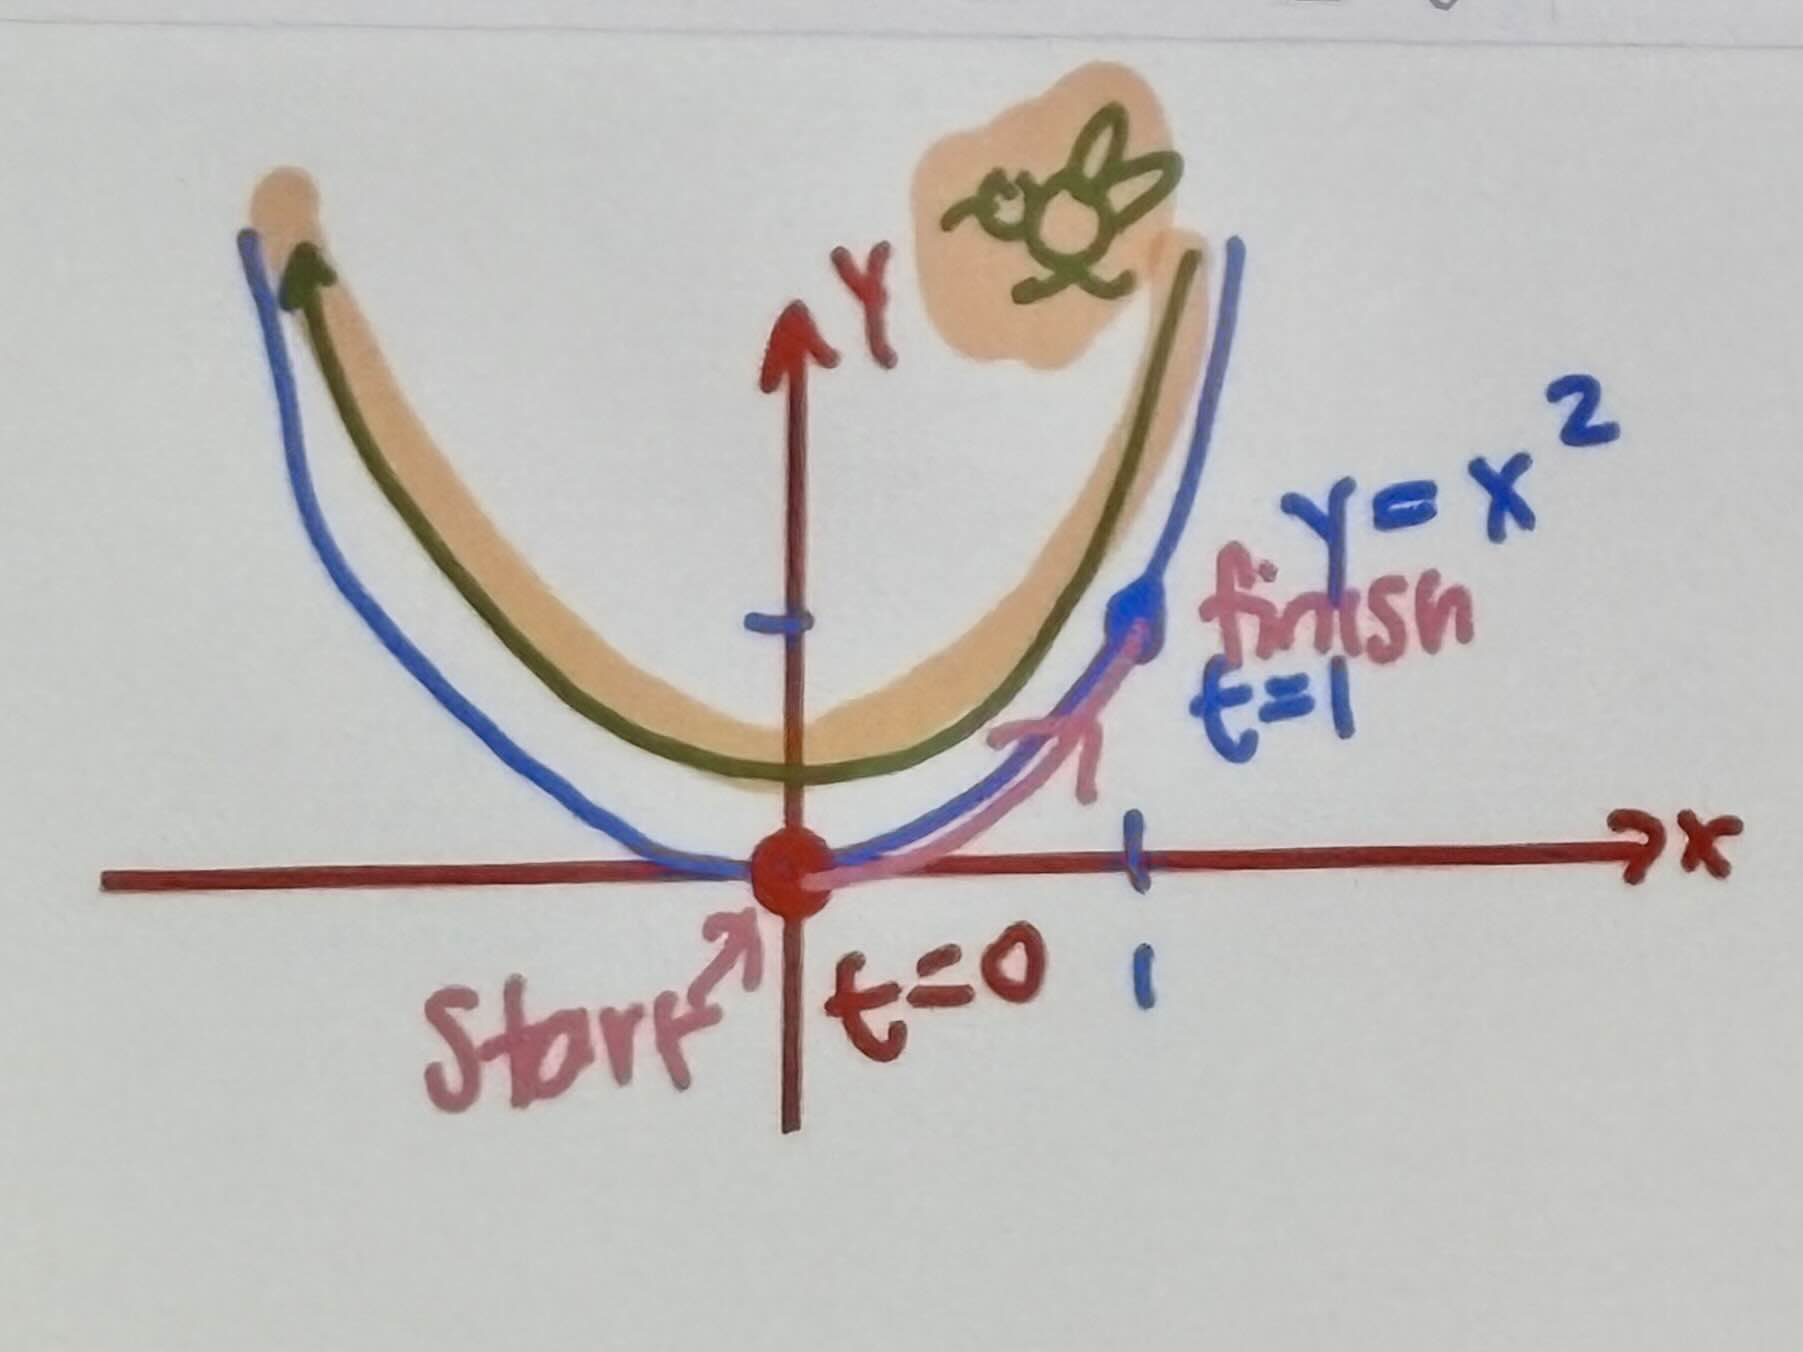
\includegraphics[width=0.6\textwidth]{parabola.jpg}
\caption{Graph of a parabola: $y = x^2$}
\label{fig:parabola}
\end{figure}

\begin{tcolorbox}[colframe=ForestGreen, colback=green!5!white, title=Parametric Equation Form]
Parametric equations are of the form:
\[ x = f(t), \quad y = g(t), \quad t \in \mathbb{R} \]
\end{tcolorbox}

For example:
\[ x = t, \quad y = t^2, \quad t \in \mathbb{R} \]
This yields points such as:
\[ (1, 1), \quad (0, 0), \quad (-1, 1) \]

Alternatively:
\[ x = -t, \quad y = t^2, \quad t \in \mathbb{R} \]
This yields points such as:
\[ (-1, 1), \quad (0, 0) \]

\section*{Drawing Parametric Equations}

\begin{tcolorbox}[colframe=RedOrange, colback=orange!5!white, title=Methods to Sketch Parametric Equations]
Two methods are commonly used to sketch parametric equations:
\begin{itemize}
    \item Use a table of values for manual computation.
    \item Convert to a Cartesian equation (eliminate $t$) and sketch the graph, if possible.
\end{itemize}
\end{tcolorbox}

\subsection*{Example}
\begin{tcolorbox}[colframe=RoyalBlue, colback=blue!5!white, title=Example Problem]
Sketch $x = t^2, y = t^3$ for $-\infty < t < \infty$.
\end{tcolorbox}

\begin{table}[H]
\centering
\begin{tabular}{|c|c|c|c|}
\hline
$t$ & $x = t^2$ & $y = t^3$ & $(x, y)$ \\
\hline
2 & 4 & 8 & (4, 8) \\
\hline
1 & 1 & 1 & (1, 1) \\
\hline
0 & 0 & 0 & (0, 0) \\
\hline
-1 & 1 & -1 & (1, -1) \\
\hline
-2 & 4 & -8 & (4, -8) \\
\hline
\end{tabular}
\caption{Table of values for $x = t^2, y = t^3$}
\end{table}

\begin{figure}[H]
\centering
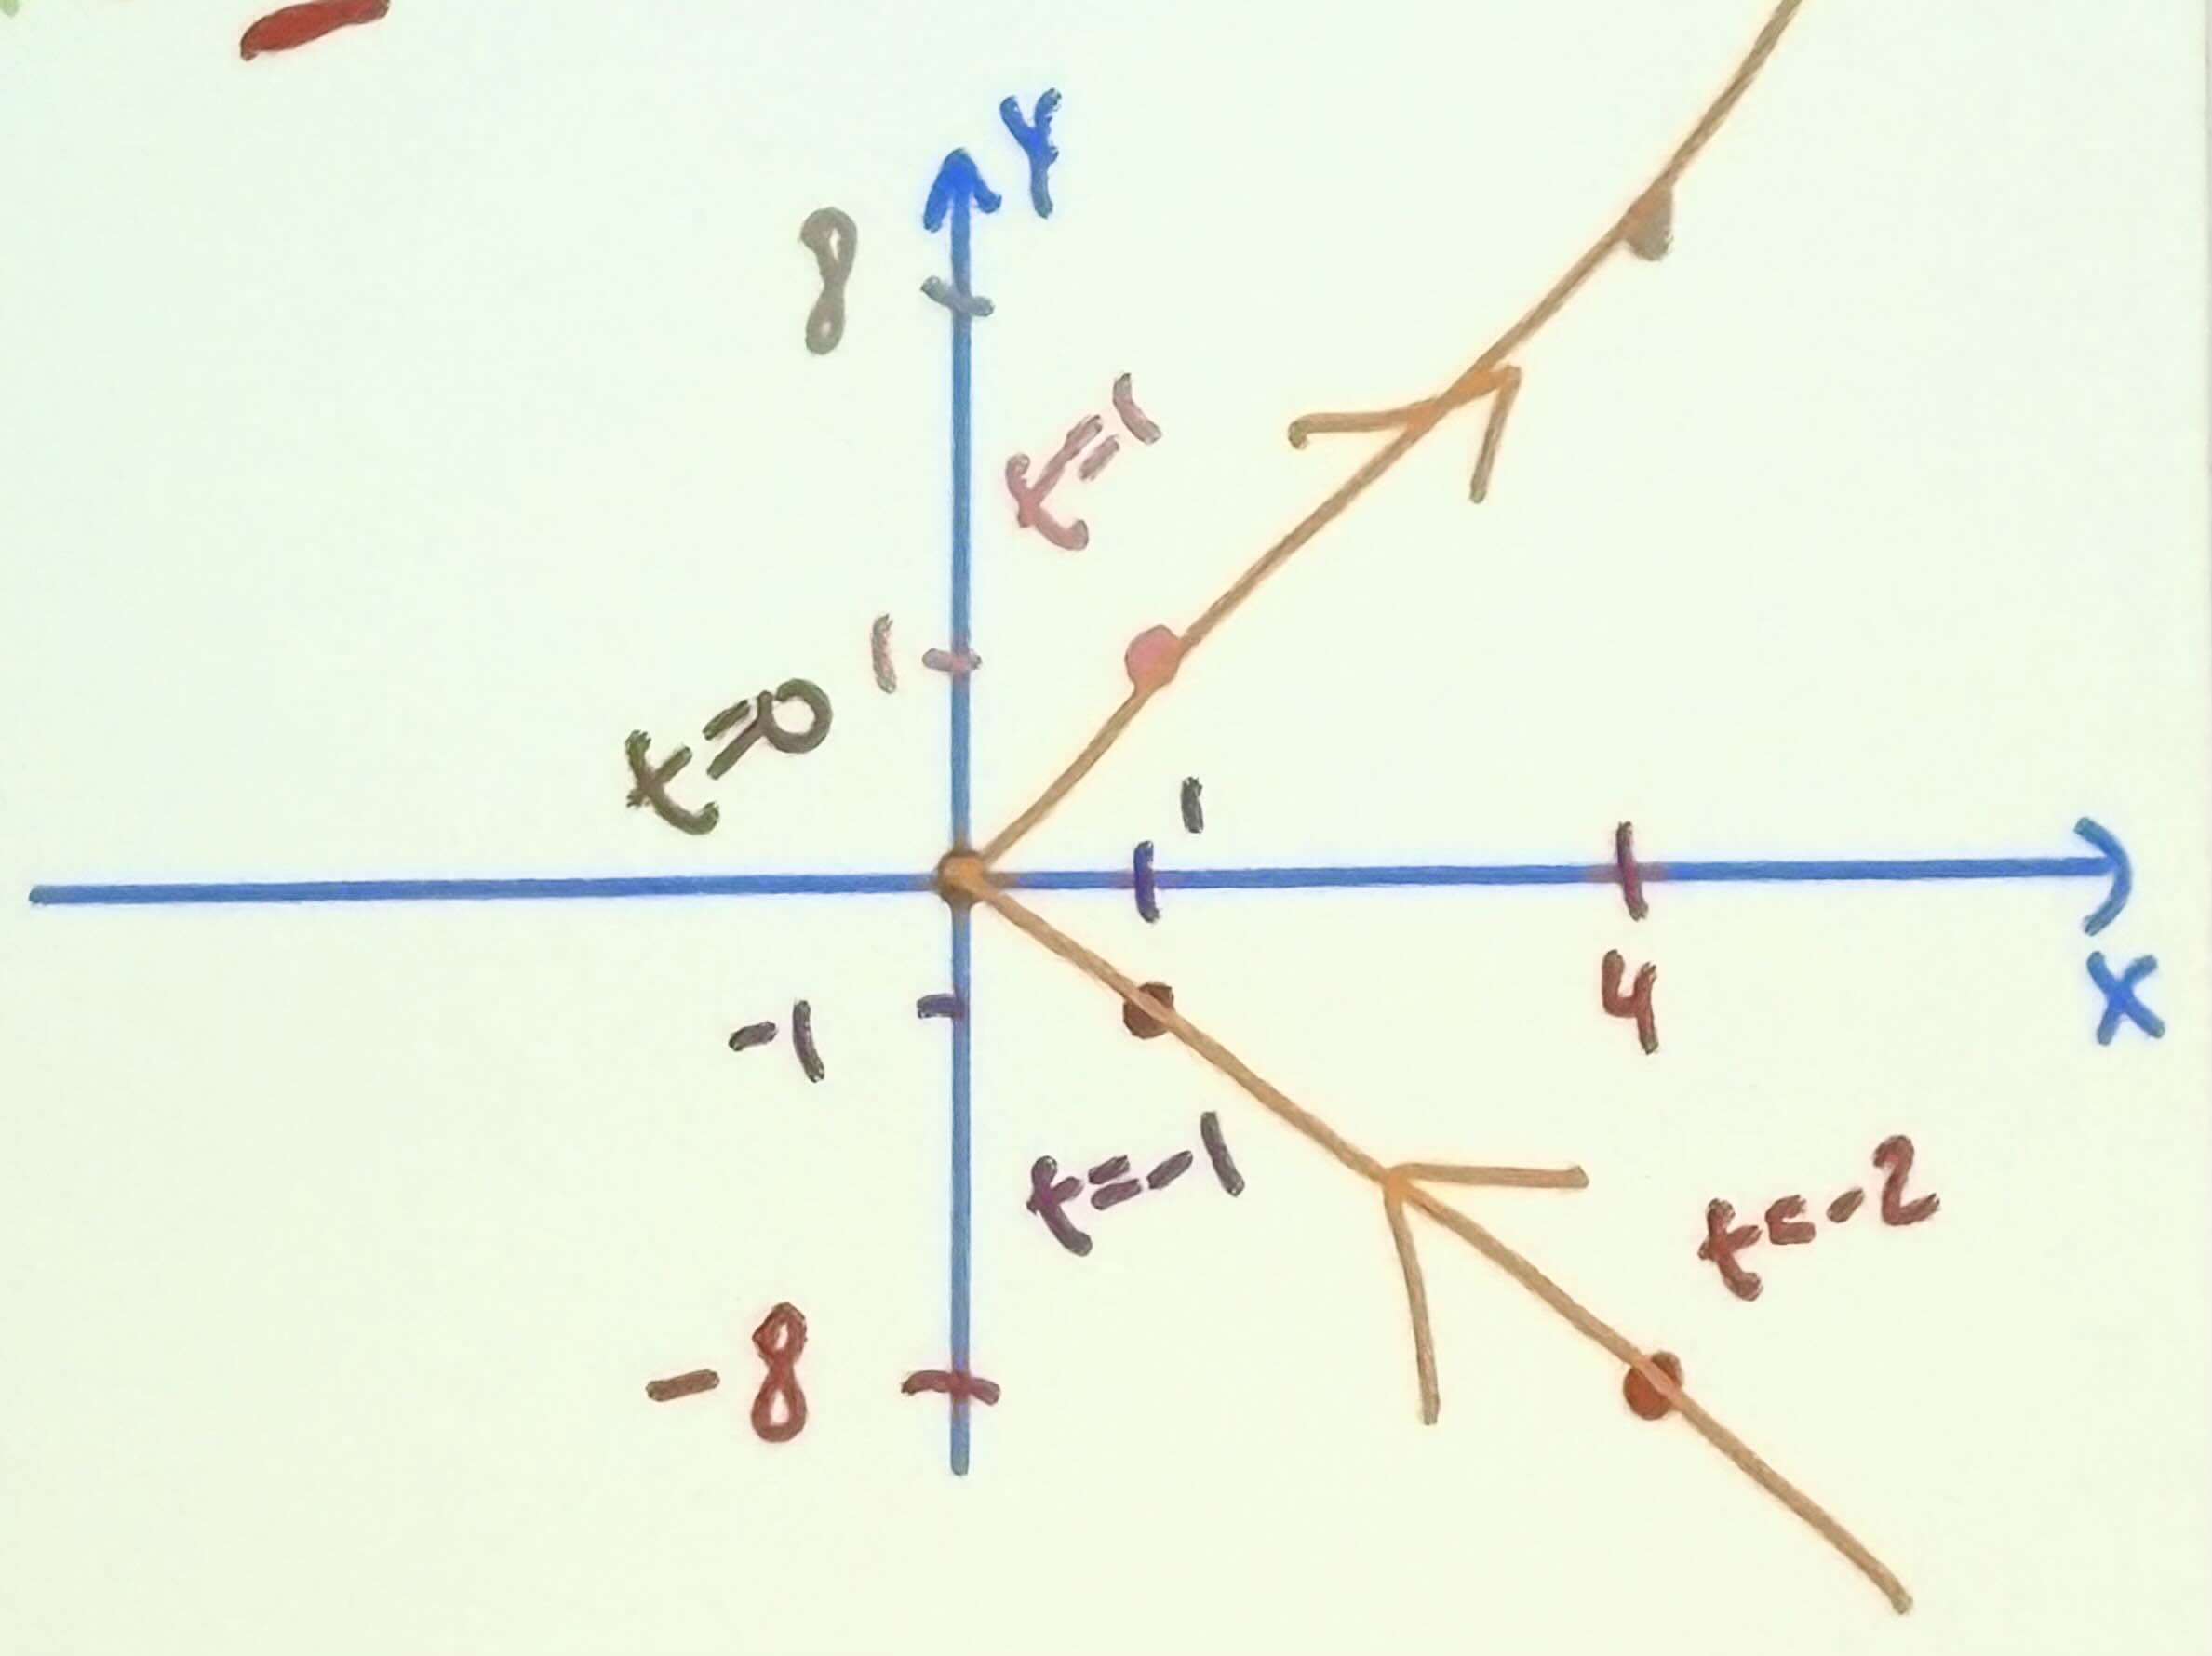
\includegraphics[width=0.4\textwidth]{sketching_example1.jpg}
\caption{Sketch of $x = t^2, y = t^3$}
\label{fig:sketch_example1}
\end{figure}

\section*{Other Examples}

\begin{tcolorbox}[colframe=RoyalPurple, colback=purple!5!white, title=Advanced Example]
A Cartesian equation is given by:
\[ \begin{aligned}
    x &= t^2, \\
    y &= t^3.
\end{aligned} \]
From these, we derive:
\[ \begin{aligned}
    x^3 &= (t^2)^3 = t^6, \\
    y^2 &= (t^3)^2 = t^6.
\end{aligned} \]
Thus, we have:
\[ x^3 = t^6 = y^2 \implies x^3 = y^2. \]
Rewriting $y^2 = x^3$, we solve for $y$:
\[ y = \pm x^{\frac{3}{2}}, \]
which gives the two solutions:
\[ y = x^{\frac{3}{2}} \quad \text{and} \quad y = -x^{\frac{3}{2}}. \]
\end{tcolorbox}

\end{document}
